\documentclass[a4paper,12pt]{article}
%%%%%%%%%%%%%%%%%%%%%%%%%%%%%%%%%%%%%%%%%%%%%%%%%%%%%%%%%%%%%%%%%%%%%%%%%%%%%%%%%%%%%%%%%%%%%%%%%%%%%%%%%%%%%%%%%%%%%%%%%%%%%%%%%%%%%%%%%%%%%%%%%%%%%%%%%%%%%%%%%%%%%%%%%%%%%%%%%%%%%%%%%%%%%%%%%%%%%%%%%%%%%%%%%%%%%%%%%%%%%%%%%%%%%%%%%%%%%%%%%%%%%%%%%%%%
\usepackage{eurosym}
\usepackage{vmargin}
\usepackage{amsmath}
\usepackage{graphics}
\usepackage{epsfig}
\usepackage{subfigure}
\usepackage{fancyhdr}

\setcounter{MaxMatrixCols}{10}
%TCIDATA{OutputFilter=LATEX.DLL}
%TCIDATA{Version=5.00.0.2570}
%TCIDATA{<META NAME="SaveForMode"CONTENT="1">}
%TCIDATA{LastRevised=Wednesday, February 23, 201113:24:34}
%TCIDATA{<META NAME="GraphicsSave" CONTENT="32">}
%TCIDATA{Language=American English}

\pagestyle{fancy}
\setmarginsrb{20mm}{0mm}{20mm}{25mm}{12mm}{11mm}{0mm}{11mm}
\lhead{MA4128} \rhead{Kevin O'Brien} \chead{Week 6} %\input{tcilatex}

\begin{document}

\tableofcontents
\newpage

% http://www.norusis.com/pdf/SPC_v13.pdf
\section{Review of Last Class}
\begin{itemize}
\item Cluster analysis is a convenient method for identifying homogenous groups of
objects called clusters. Objects (or cases, observations) in a specific cluster share
many characteristics, but are very dissimilar to objects not belonging to that cluster.
\item  There are three cluster analysis approaches: hierarchical methods,
partitioning methods (more precisely, k-means), and two-step clustering,
which is largely a combination of the first two methods. In the last class we looked as hierarchical clustering analysis.
\item Each of these procedures
follows a different approach to grouping the most similar objects into a cluster and
to determining each object’s cluster membership.
\item Some approaches – most notably hierarchical methods – require us to specify how similar or different objects
    are in order to identify different clusters. Most software packages, such as SPSS, calculate a measure
of (dis)similarity by estimating the distance between pairs of objects. Objects with
smaller distances between one another are more similar, whereas objects with larger
distances are more dissimilar.
\item An important problem in the application of cluster analysis is the decision
regarding how many clusters should be derived from the data. This question is
explored in the next step of the analysis. Sometimes, however,
number of segments that have to be derived from the data will be known in advance.
\item
By choosing a specific clustering procedure, we determine how clusters are to be
formed. (This always involves optimizing some kind of criterion, such as minimizing
the within-cluster variance (i.e., the clustering variables’ overall variance of
objects in a specific cluster), or maximizing the distance between the objects or
clusters). The procedure could also address the question of how to determine the
(dis)similarity between objects in a newly formed cluster and the remaining objects
in the dataset.
\item
Hierarchical clustering procedures are characterized by the tree-like structure
established in the course of the analysis. Most hierarchical techniques fall into a
category called agglomerative clustering. In this category, clusters are consecutively
formed from objects. Initially, this type of procedure starts with each object
representing an individual cluster. These clusters are then sequentially merged
according to their similarity. First, the two most similar clusters (i.e., those with
the smallest distance between them) are merged to form a new cluster at the bottom
of the hierarchy. In the next step, another pair of clusters is merged and linked to a
higher level of the hierarchy, and so on. This allows a hierarchy of clusters to be
established from the bottom up.
\item A cluster hierarchy can also be generated top-down. In this divisive clustering,
all objects are initially merged into a single cluster, which is then gradually split up. Divisive procedures are quite rarely used in practice. We therefore
concentrate on the agglomerative clustering procedures.
\item This means that if an object is assigned
to a certain cluster, there is no possibility of reassigning this object to another
cluster. This is an important distinction between these types of clustering and
partitioning methods such as \textbf{\textit{k-means}}.
\newpage
\item There are various measures to express (dis)similarity between pairs of objects.
A straightforward way to assess two objects’ proximity is by drawing a straight line
between them.This type of distance is also referred to as
\textbf{\textit{Euclidean distance}} (or straight-line distance) and is the most commonly used type
when it comes to analyzing ratio or interval-scaled data.
\begin{figure}[h!]
\begin{center}
  % Requires \usepackage{graphicx}
  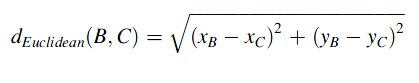
\includegraphics[scale=0.6]{EuclidDistance1.jpg}\\
\end{center}
\end{figure}

The Euclidean distance is the square root of the sum of the squared differences in
the variables’ values. Suppose B and C were positioned as $(7,6)$ and $(6,5)$ respectively.
\begin{figure}[h!]
\begin{center}
  % Requires \usepackage{graphicx}
  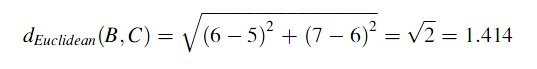
\includegraphics[scale=0.6]{EuclidDistance2.jpg}\\
\end{center}
\end{figure}

This distance corresponds to the length of the line that connects objects B and C.
In this case, we only used two variables but we can easily add more under the root
sign in the formula. However, each additional variable will add a dimension to our
research problem (e.g., with ten clustering variables, we have to deal with ten
dimensions), making it impossible to represent the solution graphically.

\item  The \textbf{\textit{Squared Euclidean distance}} uses the same equation as the Euclidean distance metric, but does not take the square root. In the previous example, the squared Euclidean distance between B and C is 2.
As a result, clustering with the Squared Euclidean distance is computationally faster than clustering with the regular Euclidean distance.

\item We can compute the distance between all other pairs of objects. All
these distances are usually expressed by means of a \textit{\textbf{distance matrix}}. In this distance
matrix, the non-diagonal elements express the distances between pairs of objects
and zeros on the diagonal (the distance from each object to itself is, of course, 0). In
our example, the distance matrix is an $8 \times 8$ table with the lines and rows
representing the objects under consideration.
\begin{figure}[h!]
\begin{center}
  % Requires \usepackage{graphicx}
  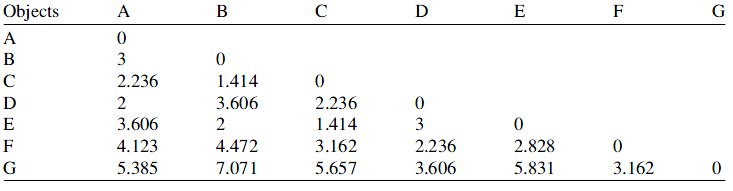
\includegraphics[scale=0.6]{DistanceMatrix.jpg}\\
\end{center}
\end{figure}

\item There are also alternative distance measures: The \textbf{\textit{Manhattan distance}} or city-block distance uses the sum of the variables’ absolute differences. This is often called the Manhattan metric
as it is akin to the walking distance between two points in a city like New York’s
Manhattan district, where the distance equals the number of blocks in the directions
North-South and East-West. Using the points B and C that we used previously, the manhattan distance is computed as follows:
\begin{figure}[h!]
\begin{center}
  % Requires \usepackage{graphicx}
  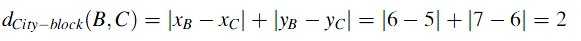
\includegraphics[scale=0.6]{Manhattan.jpg}\\
\end{center}
\end{figure}


\item When working with metric (or ordinal) data, researchers frequently use
the \textbf{\textit{Chebychev distance}}, which is the maximum of the absolute difference in the
clustering variables’ values. For B and C, this result is:

\begin{figure}[h!]
\begin{center}
  % Requires \usepackage{graphicx}
  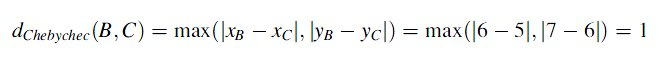
\includegraphics[scale=0.6]{Chebyshev.jpg}\\
\end{center}
\end{figure}

\item There are other distance measures such as the Angular, Canberra or Mahalanobis
distance. In many situations, the \textbf{\textit{Mahalanobis
distance}} is desirable as this measure compensates for \textbf{\textit{multi-collinearity}}
between the clustering variables. However, it is unfortunately not menu-accessible
in SPSS.
\item
In statistics, the occurrence of several  variables in a multiple regression model are \textbf{closely correlated} to one another, and carrying the same information, more or less. Multi-collinearity can cause strange results when attempting to study how well individual independent variables contribute to an understanding of the dependent variable, often undermining the analysis.

\item In many analysis tasks, the variables under consideration are measured on
different scales or levels. This would
clearly distort any clustering analysis results. We can resolve this problem by \textbf{\textit{standardizing}}
the data prior to the analysis.

\item Different standardization methods are available, such as the simple \textbf{\textit{z standardization}},
which re-scales each variable to have a mean of 0 and a standard deviation of 1.

\item In most situations, however, \textbf{\textit{standardization by range}}(e.g., to a
range of 0 to 1 or -1 to 1) is preferable. We recommend standardizing the data
in general, even though this procedure can potentially reduce or inflate the variables’ influence
on the clustering solution.

\item A commonly used approach in hierarchical clustering is \textbf{\textit{Ward’s linkage method}}.
This approach does not combine the two most similar objects successively. Instead,
those objects whose merger increases the overall within-cluster variance to the
smallest possible degree, are combined. If you expect somewhat equally sized
clusters and the data set does not include outliers, you should always use Ward’s
method.

We will use the Ward's linkage method for laboratory exercises.

\item Other most popular
agglomerative clustering procedures include the following:
\begin{description}
\item[Single linkage (nearest neighbor)]: The distance between two clusters corresponds
to the shortest distance between any two members in the two clusters.
\begin{figure}[h!]
\begin{center}
  % Requires \usepackage{graphicx}
  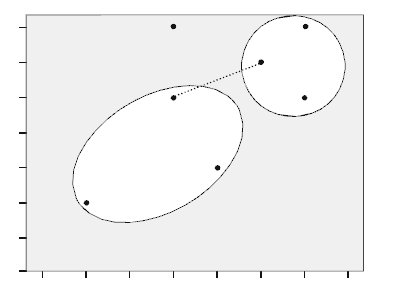
\includegraphics[scale=0.4]{Link1.jpg}\\
\end{center}
\end{figure}
\item[Complete linkage (furthest neighbor)]: The oppositional approach to single
linkage assumes that the distance between two clusters is based on the longest
distance between any two members in the two clusters.
\begin{figure}[h!]
\begin{center}
  % Requires \usepackage{graphicx}
  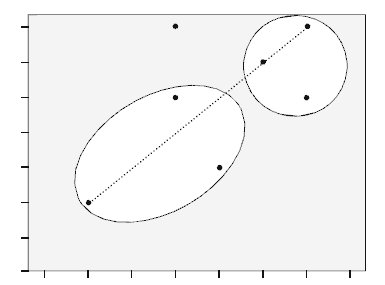
\includegraphics[scale=0.4]{Link2.jpg}\\
\end{center}
\end{figure}
\item[Average linkage] : The distance between two clusters is defined as the average
distance between all pairs of the two clusters’ members.
\begin{figure}[h!]
\begin{center}
  % Requires \usepackage{graphicx}
  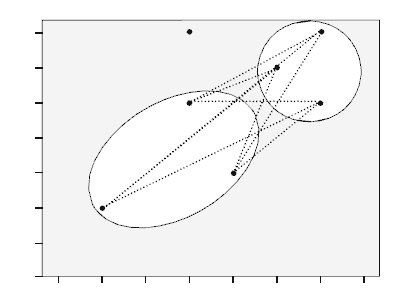
\includegraphics[scale=0.4]{Link3.jpg}\\
\end{center}
\end{figure}
\newpage
\item[Centroid] : In this approach, the geometric center (centroid) of each cluster is
computed first. The distance between the two clusters equals the distance between
the two centroids.
\begin{figure}[h!]
\begin{center}
  % Requires \usepackage{graphicx}
  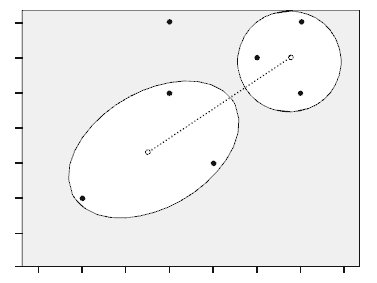
\includegraphics[scale=0.4]{Link4.jpg}\\
\end{center}
\end{figure}
\end{description}
Each of these linkage algorithms can yield totally different results when used on the same data set, as each has its specific properties. As the single linkage algorithm is based on minimum distances, it tends to form one large cluster with the other clusters containing only one or few objects each. We can make use of this \textbf{\textit{chaining effect}} to detect outliers, as these will be merged with the remaining objects – usually at very large distances – in the last steps of the analysis. Generally, single linkage is considered the most versatile algorithm.

Conversely, the complete linkage method is strongly affected by outliers, as it is based on maximum distances. Clusters produced by this method are likely to be rather compact and tightly clustered. The average linkage and centroid algorithms tend to produce clusters with rather low within-cluster variance and similar sizes.
However, both procedures are affected by outliers, though not as much as complete linkage.

An understanding of linkage method's other than than Ward method will be expected in the end of year examination.

\item A common way to visualize the cluster analysis’s progress is by drawing a
dendrogram, which displays the distance level at which there was a combination
of objects and clusters.
Here is an example of a dendrogram (which corresponds to the example in the next section of material.


\begin{figure}[h!]
\begin{center}
  % Requires \usepackage{graphicx}
  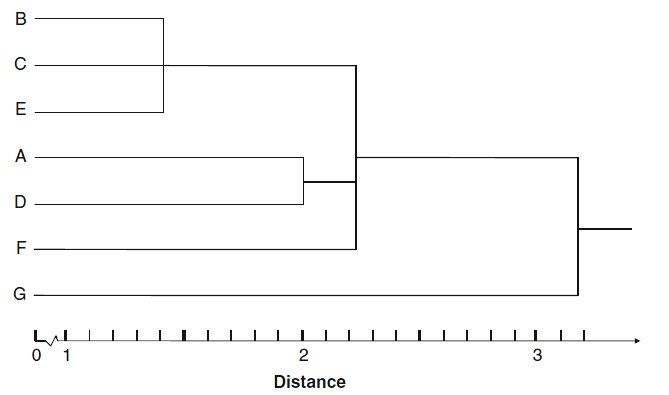
\includegraphics[scale=0.6]{Dendrogram.jpg}\\
\end{center}
\end{figure}

\item An important question is how to decide on the number of
clusters to retain from the data. Unfortunately, hierarchical methods provide only
very limited guidance for making this decision. The only meaningful indicator
relates to the distances at which the objects are combined. Similar to factor
analysis’s scree plot, we can seek a solution in which an additional combination
of clusters or objects would occur at a greatly increased distance. This raises the
issue of what a great distance is, of course. For this purpose, we can make use of the dendrogram.

\item In constructing the dendrogram, SPSS rescales the distances to a range
of 0–25; that is, the last merging step to a one-cluster solution takes place at a
(rescaled) distance of 25. The rescaling often lengthens the merging steps, thus
making breaks occurring at a greatly increased distance level more obvious.
Despite this, this distance-based decision rule does not work very well in all
cases.

It is often difficult to identify where the break actually occurs. This is also
the case in our example above. By looking at the dendrogram, we could justify
a two-cluster solution ([A,B,C,D,E,F] and [G]), as well as a five-cluster solution
([B,C,E], [A], [D], [F], [G]).


\end{itemize}
\newpage
\section{Clustering Algorithm}
To better understand how a clustering algorithm works, let’s manually examine
some of the single linkage procedure’s calculation steps. We start off by looking at
the initial (Euclidean) distance matrix displayed previously.

\begin{figure}[h!]
\begin{center}
  % Requires \usepackage{graphicx}
  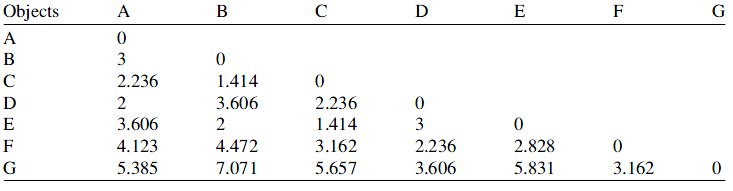
\includegraphics[scale=0.6]{DistanceMatrix.jpg}\\
\end{center}
\end{figure}

\begin{itemize}
\item In the very first step, the two
objects exhibiting the smallest distance in the matrix are merged. Note that we
always merge those objects with the smallest distance, regardless of the clustering
procedure (e.g., single or complete linkage). (N.B. In the following example, ties will be broken at random.)
\item As we can see, this happens to two
pairs of objects, namely B and C (d(B, C) = 1.414), as well as C and E (d(C, E) =
1.414). In the next step, we will see that it does not make any difference whether we
first merge the one or the other, so let’s proceed by forming a new cluster, using
objects B and C.
\begin{figure}[h!]
\begin{center}
  % Requires \usepackage{graphicx}
  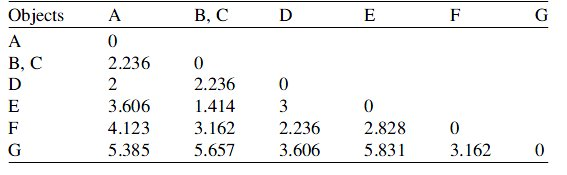
\includegraphics[scale=0.6]{DistanceMatrix2.jpg}\\
\end{center}
\end{figure}
\item Having made this decision, we then form a new distance matrix by considering
the single linkage decision rule as discussed above. According to this rule, the
distance from, for example, object A to the newly formed cluster is the minimum of
d(A, B) and d(A, C). As d(A, C) is smaller than d(A, B), the distance from A to the
newly formed cluster is equal to d(A, C); that is, 2.236.
\item We also compute the
distances from cluster [B,C] (clusters are indicated by means of squared brackets)
to all other objects (i.e. D, E, F, G) and simply copy the remaining distances – such
as d(E, F) – that the previous clustering has not affected.
\begin{figure}[h!]
\begin{center}
  % Requires \usepackage{graphicx}
  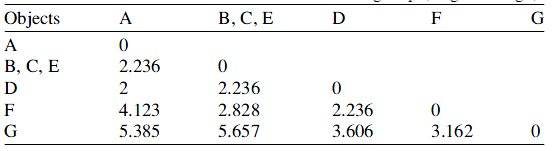
\includegraphics[scale=0.6]{DistanceMatrix3.jpg}\\
\end{center}
\end{figure}
\item Continuing the clustering procedure, we simply repeat the last step by merging
the objects in the new distance matrix that exhibit the smallest distance (in this case,
the newly formed cluster [B, C] and object E) and calculate the distance from this
cluster to all other objects.
\begin{figure}[h!]
\begin{center}
  % Requires \usepackage{graphicx}
  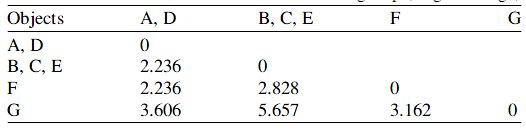
\includegraphics[scale=0.6]{DistanceMatrix4.jpg}\\
\end{center}
\end{figure}
\item We continue in the same fashion until one cluster is left. By following the single linkage procedure, the last steps involve the merger
of cluster [A,B,C,D,E,F] and object G at a distance of 3.162.
\begin{figure}[h!]
\begin{center}
  % Requires \usepackage{graphicx}
  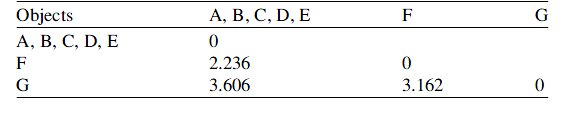
\includegraphics[scale=0.6]{DistanceMatrix5.jpg}\\
\end{center}
\end{figure}
\begin{figure}[h!]
\begin{center}
  % Requires \usepackage{graphicx}
  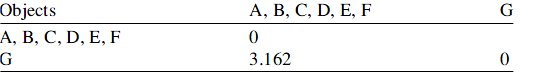
\includegraphics[scale=0.6]{DistanceMatrix6.jpg}\\
\end{center}
\end{figure}
\end{itemize}
\newpage


\section{K-Means Clustering}
\begin{itemize}
\item Hierarchical clustering requires a distance or similarity matrix between all pairs of cases. That's an extremely large matrix if you have tens of thousands of cases in your data file.

\item A clustering method that doesn't require computation of all possible distances is k-means clustering. It differs from hierarchical clustering in several ways. You have to know in advance the number of clusters you want. You can't get solutions for a range of cluster numbers unless you rerun the analysis for each different number of clusters.

\item The algorithm repeatedly reassigns cases to clusters, so the same case can move from cluster to cluster during the analysis. In agglomerative hierarchical clustering, on the other hand, cases are added only to existing clusters. They are forever captive in their cluster, with a widening circle of ``neighbours".

\item The algorithm is called \textbf{k-means}, where \textbf{k} is the number of clusters you want, since a case is assigned to the cluster for which its distance to the cluster mean is the smallest.

\item The k-means algorithm follows an entirely different concept than the hierarchical methods
discussed before. This algorithm is not based on distance measures such as
Euclidean distance or city-block distance, but uses the \textbf{\textit{within-cluster variation}} as a measure to form homogenous clusters. Specifically, the procedure aims at segmenting
the data in such away that the within-cluster variation isminimized.Consequently,we
do not need to decide on a distance measure in the first step of the analysis.

\item The action in the algorithm centers around finding the k-means. You start out with an initial set of means and classify cases based on their distances to the centers.

\item Next, you compute the cluster means again, using the cases that are assigned to the cluster; then, you reclassify all cases based on the new set of means. You keep repeating this step until cluster means don't change much between successive steps.

\item Finally, you calculate the means of the clusters once again and assign the cases to their permanent clusters.
\end{itemize}
\subsection{Performance of k-means clustering}
Generally, k-means is superior to hierarchical methods as it is less affected by
outliers and the presence of irrelevant clustering variables. Furthermore, k-means
can be applied to very large data sets, as the procedure is less computationally
demanding than hierarchical methods. In fact, we suggest definitely using k-means
for sample sizes above 500, especially if many clustering variables are used. From
a strictly statistical viewpoint, k-means should only be used on interval or ratio-scaled
data as the procedure relies on Euclidean distances. However, the procedure is
routinely used on ordinal data as well, even though there might be some distortions.

One problem associated with the application of k-means relates to the fact that
the researcher has to pre-specify the number of clusters to retain from the data. This
makes k-means less attractive to some and still hinders its routine application in
practice.
\end{document}

